\documentclass{article}

\usepackage{tikz}
\usetikzlibrary{patterns, arrows.meta}

\begin{document}
	
	\begin{center}
		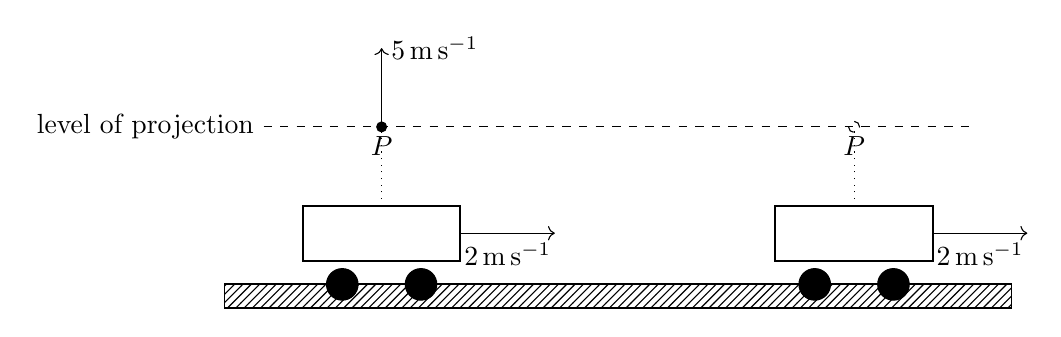
\begin{tikzpicture}[scale=1]
			
			% Ground line
			\draw[thick] (0,0) -- (10,0);
			
			% Ground shading
			\draw[pattern=north east lines] (0,-0.3) rectangle (10,0);
			
			% LEFT CAR
			\draw[thick] (1,0.3) rectangle (3,1);
			\draw[fill=black] (1.5,0) circle (0.2);
			\draw[fill=black] (2.5,0) circle (0.2);
			
			% RIGHT CAR
			\draw[thick] (7,0.3) rectangle (9,1);
			\draw[fill=black] (7.5,0) circle (0.2);
			\draw[fill=black] (8.5,0) circle (0.2);
			
			% Dashed horizontal line (level of projection)
			\draw[dashed] (0.5,2) -- (9.5,2);
			\node[left] at (0.5,2) {level of projection};
			
			% Vertical dotted guides
			\draw[dotted] (2,1) -- (2,2);
			\draw[dotted] (8,1) -- (8,2);
			
			% Projectile point (left)
			\fill (2,2) circle (2pt);
			\node[below] at (2,2) {$P$};
			
			% Projectile point (right, dashed circle)
			\draw[dashed] (8,2) circle (2pt);
			\node[below] at (8,2) {$P$};
			
			% Vertical velocity (5 m/s)
			\draw[->] (2,2) -- (2,3);
			\node[right] at (2,3) {$5\,\mathrm{m\,s^{-1}}$};
			
			% Horizontal velocity arrows (cars)
			\draw[->] (3,0.65) -- (4.2,0.65);
			\node[below] at (3.6,0.65) {$2\,\mathrm{m\,s^{-1}}$};
			
			\draw[->] (9,0.65) -- (10.2,0.65);
			\node[below] at (9.6,0.65) {$2\,\mathrm{m\,s^{-1}}$};
			
		\end{tikzpicture}
	\end{center}
	
\end{document}